\section{Evaluation}
\label{sec.evaluation}

\subsection{Evaluation Methodology}
We want to evaluate our metric, and new architecture and designs that came from our metric. 
The methodology is we implement one new system Lind, using our new design, and compare it 
with other systems not using our design. The comparison results will show if our system is better, 
which in turn will show if our metric is effective. 

\subsection{The Comparison Results and Analysis}
We conducted comparison between Lind and other systems, which were Native Linux, 
VirtualBox and Graphene. Native Linux was used as a baseline, while VirtualBox and Graphene
were both competitive systems that also aimed at user application isolation.

\subsubsection{Security Evaluation}
Since Lind aims at achieving a very secure system, and leverages our metric by using its 
security-prioritized guidelines. We first focused on comparing the security of each of the systems.

Again, we used two approaches, system call fuzzing and running user applications, to obtain the
kernel profiling data. 

We first compared the kernel trace under different environments.
The comparison results for running system call fuzzing and user applications in different systems 
are shown in Figure 5 and 6.

\begin{figure}[h]
\centering
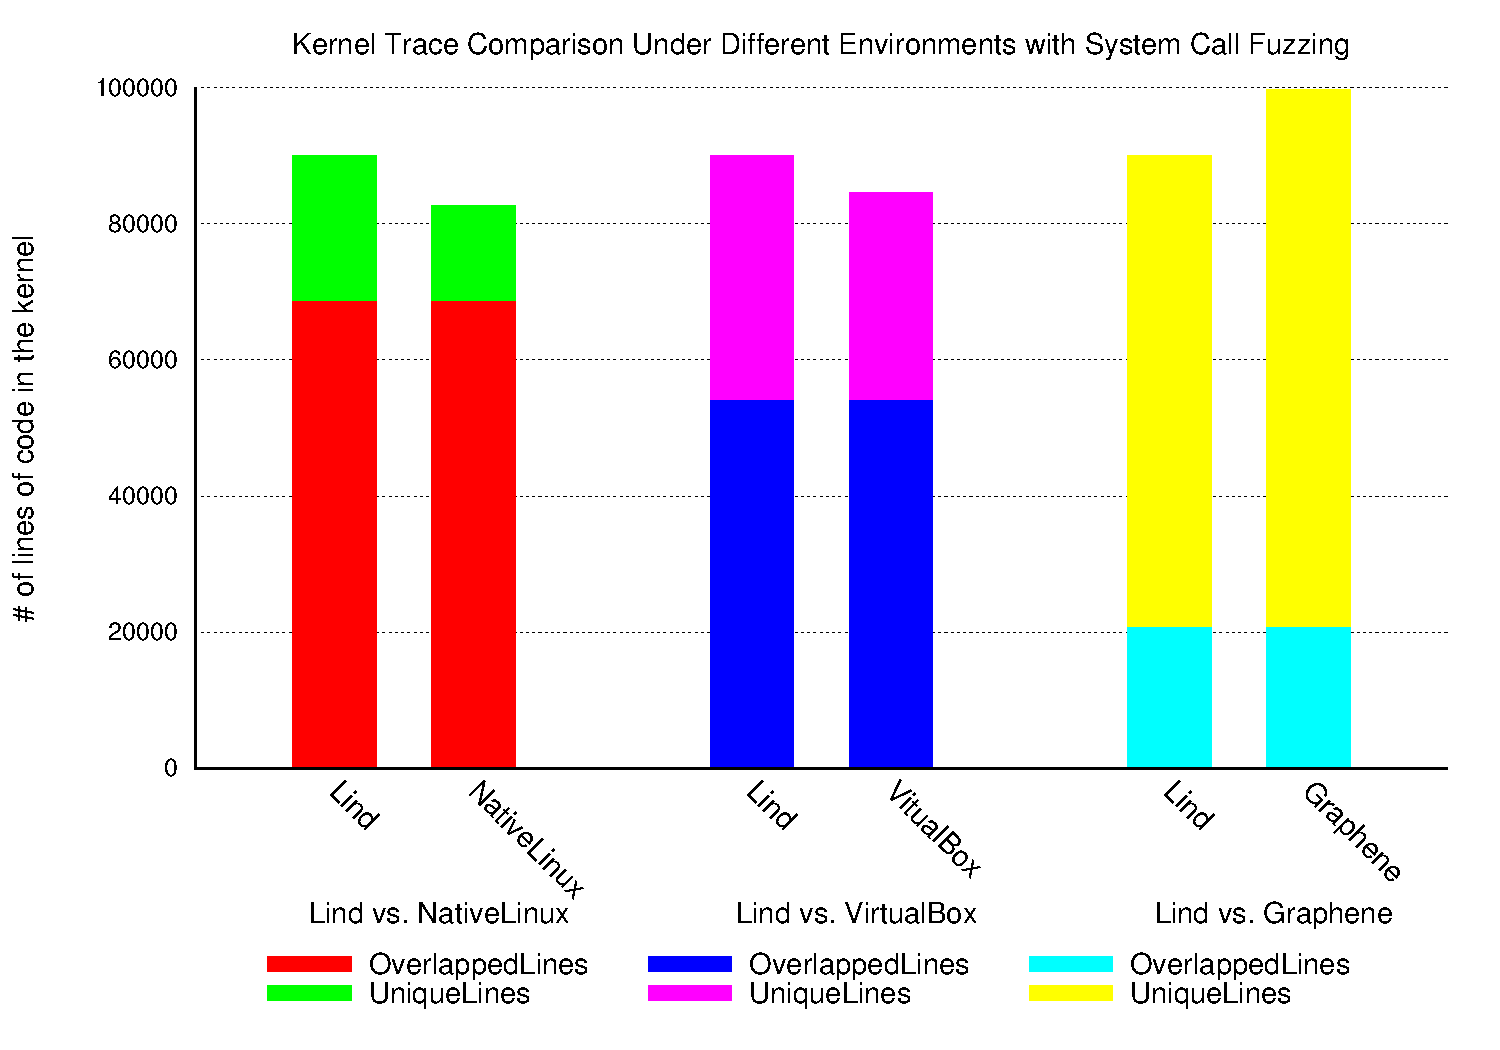
\includegraphics[width=1.0\columnwidth]{diagram/lind_ccs15_diagram_03.pdf}
\caption{Kernel Trace in Different Systems with System Call Fuzzing}
\label{fig:different_systems_systemcallfuzzing_trace}
\end{figure}

\begin{figure}[h]
\centering
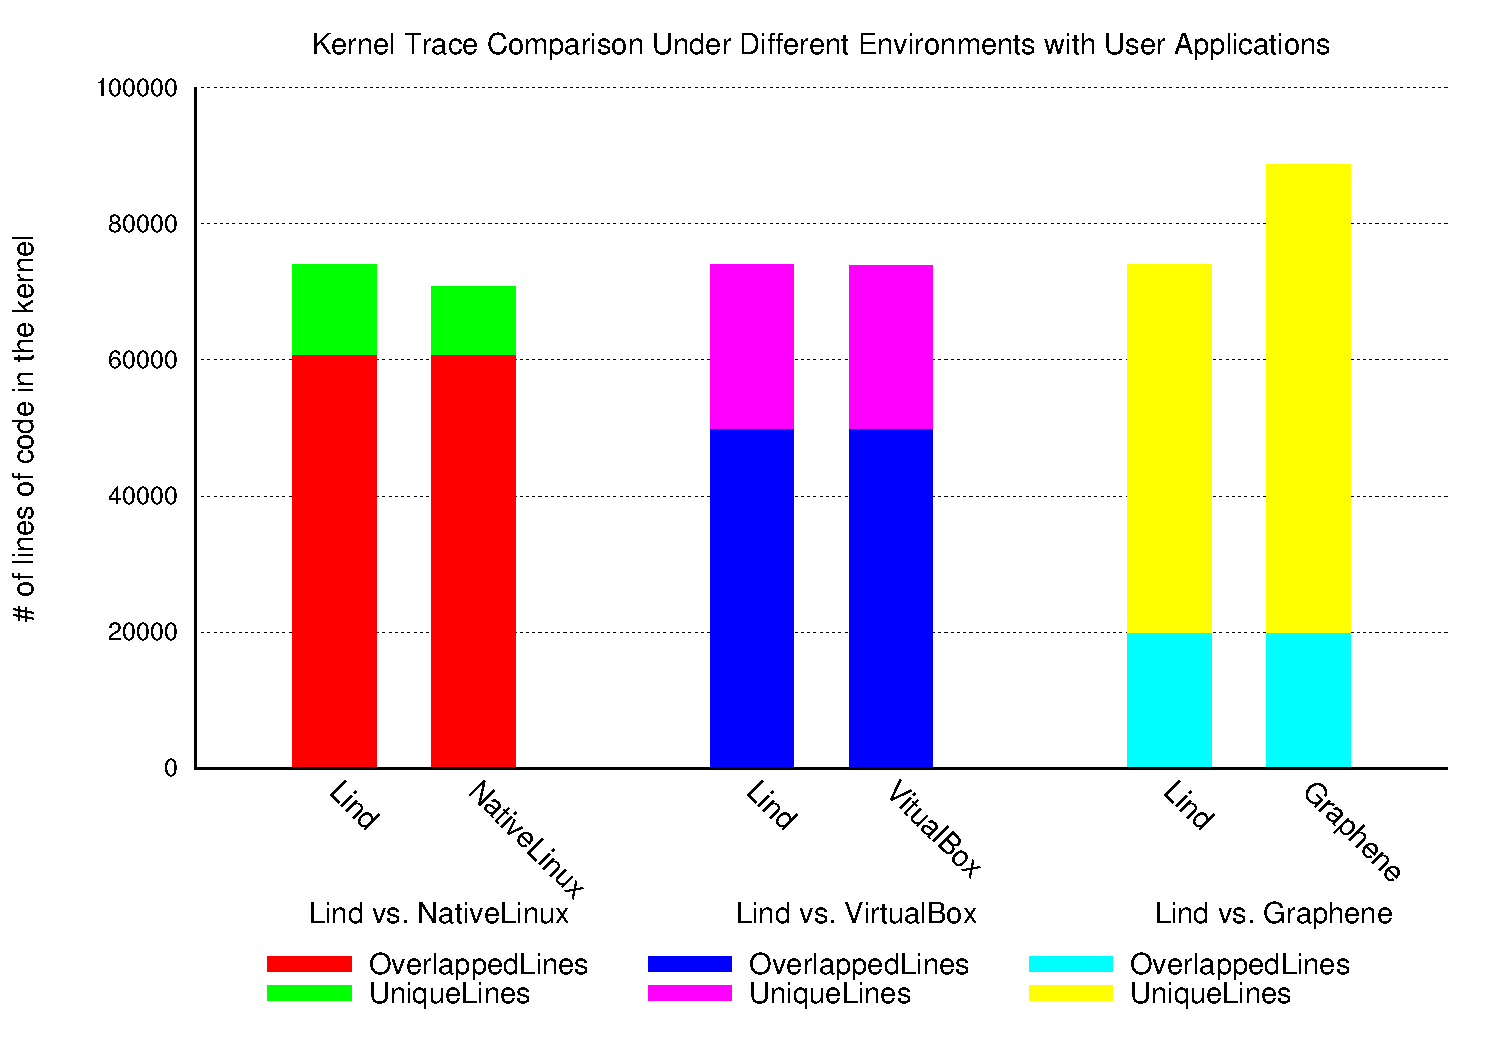
\includegraphics[width=1.0\columnwidth]{diagram/lind_ccs15_diagram_04.pdf}
\caption{Kernel Trace in Different Systems with Running User Applications}
\label{fig:different_systems_userapplications_trace}
\end{figure}

Now, we want to verify how likely it is to trigger kernel bugs in each of the environment.
We already had kernel trace generated by running system call fuzzing and user applications.
In order to check if kernel bugs might appear in those traces, we examine a list of 19 reported 
kernel bugs, and identify the kernel paths involved in triggering each of the bugs.

The list of bugs we used in our analysis is shown in Table 2.

\begin{table*}[t]
\begin{tabular*}{\textwidth}{l @{\extracolsep{\fill}} lc}
\toprule
\multicolumn{2}{c}{Kernel Bugs Examined} \\
\midrule
Vulnerability    &  Specific Type \\
\midrule
 CVE-2009-3234 \cite{CVE:20093234} & stack and heap buffer overflows \\
 CVE-2013-1828 \cite{CVE:20131828} & stack and heap buffer overflows \\
 CVE-2013-2892 \cite{CVE:20132892} & stack and heap buffer overflows \\
 CVE-2005-0736 \cite{CVE:20050736} & NULL pointer and pointer arithmetic errors \\
 CVE-2009-2698 \cite{CVE:20092698} & NULL pointer and pointer arithmetic errors \\
 CVE-2009-3002 \cite{CVE:20093002} &  memory disclosure vulnerabilities \\
 CVE-2010-4073 \cite{CVE:20104073} &  memory disclosure vulnerabilities \\
 CVE-2013-2852 \cite{CVE:20132852} &  use-after-free and format string bugs \\
 CVE-2013-4343 \cite{CVE:20134343} &  use-after-free and format string bugs \\
 CVE-2010-3437 \cite{CVE:20103437} &  signedness errors \\
 CVE-2013-2094 \cite{CVE:20132094} &  signedness errors \\
 CVE-2005-0736 \cite{CVE:20050736} &  integer overflows \\
 CVE-2010-2959 \cite{CVE:20102959} &  integer overflows \\
 CVE-2009-1527 \cite{CVE:20091527} &  race conditions \\
 CVE-2009-3547 \cite{CVE:20093547} &  race conditions \\
 CVE-2010-3904 \cite{CVE:20103904} &  missing authorization checks and poor argument sanitization\\
 CVE-2010-4347 \cite{CVE:20104347} &  missing authorization checks and poor argument sanitization\\
 CVE-2012-0946 \cite{CVE:20120946} &  missing authorization checks and poor argument sanitization\\
 CVE-2013-0268 \cite{CVE:20130268} &  missing authorization checks and poor argument sanitization\\
\bottomrule
\end{tabular*}
\caption {Kernel Bugs Examined}
\label{table:kernel_bugs}
\end{table*}

After examination of the bugs, we matched the kernel traces in different environments against the kernel traces generated 
by the bugs to verify if a bug might be triggered under each environment. 

The results for verifying which kernel bugs may be triggered under each environment is illustrated in Table 3. 

\begin{table*}[t]
\begin{tabular*}{\textwidth}{l @{\extracolsep{\fill}} cccc}
\toprule
\multicolumn{5}{c}{Possibility of Triggering Kernel Vulnerabilities} \\
\midrule
Vulnerability    &  Native Linux OS  &  Lind  &  Graphene & VirtualBox\\
\midrule
 CVE-2009-3234 \cite{CVE:20093234} & yes & no & no & no\\
 CVE-2013-1828 \cite{CVE:20131828} & no & no & yes & yes\\
 CVE-2013-2892 \cite{CVE:20132892} & yes & no & yes & yes\\
 CVE-2005-0736 \cite{CVE:20050736} & yes & yes & yes & no\\
 CVE-2009-2698 \cite{CVE:20092698} & yes & no & yes & yes\\
 CVE-2009-3002 \cite{CVE:20093002} & yes & no & yes & no\\
 CVE-2010-4073 \cite{CVE:20104073} & yes & no & yes & yes\\
 CVE-2013-2852 \cite{CVE:20132852} & yes & no & no & no\\
 CVE-2013-4343 \cite{CVE:20134343} & yes & no & no & no\\
 CVE-2010-3437 \cite{CVE:20103437} & no & no & no & no\\
 CVE-2013-2094 \cite{CVE:20132094} & no & no & yes & yes\\
 CVE-2005-0736 \cite{CVE:20050736} & no & no & yes & no\\
 CVE-2010-2959 \cite{CVE:20102959} & yes & no & yes & no\\
 CVE-2009-1527 \cite{CVE:20091527} & yes & no & yes & no\\
 CVE-2009-3547 \cite{CVE:20093547} & yes & no & yes & no\\
 CVE-2010-3904 \cite{CVE:20103904} & yes & no & no & no\\
 CVE-2010-4347 \cite{CVE:20104347} & no & no & yes & no\\
 CVE-2012-0946 \cite{CVE:20120946} & yes & no & no & yes\\
 CVE-2013-0268 \cite{CVE:20130268} & yes & no & yes & yes\\
\bottomrule
\end{tabular*}
\caption {Possibility of Triggering Kernel Vulnerabilities (``yes'': possible to trigger the bug; ``no'': not possible to trigger the bug)}
\label{table:trigger_vulnerabilities}
\end{table*}

\subsubsection{Performance Evaluation}
Besides the security evaluation, we also did performance evaluation on running applications in each of the different environment.
The purpose of this performance evaluation is to show that although system like Lind is designed and built to provide stronger
security, it can also function well with reasonable overhead. 

Comparison results for the performance evaluation are shown in Figure 7.
The results show that the overhead of running applications in Lind is acceptable, compared with other systems. 
This validates that systems designed and built using our metric can achieve the design goals, as well as function well in practice. 

\begin{figure}[h]
\centering
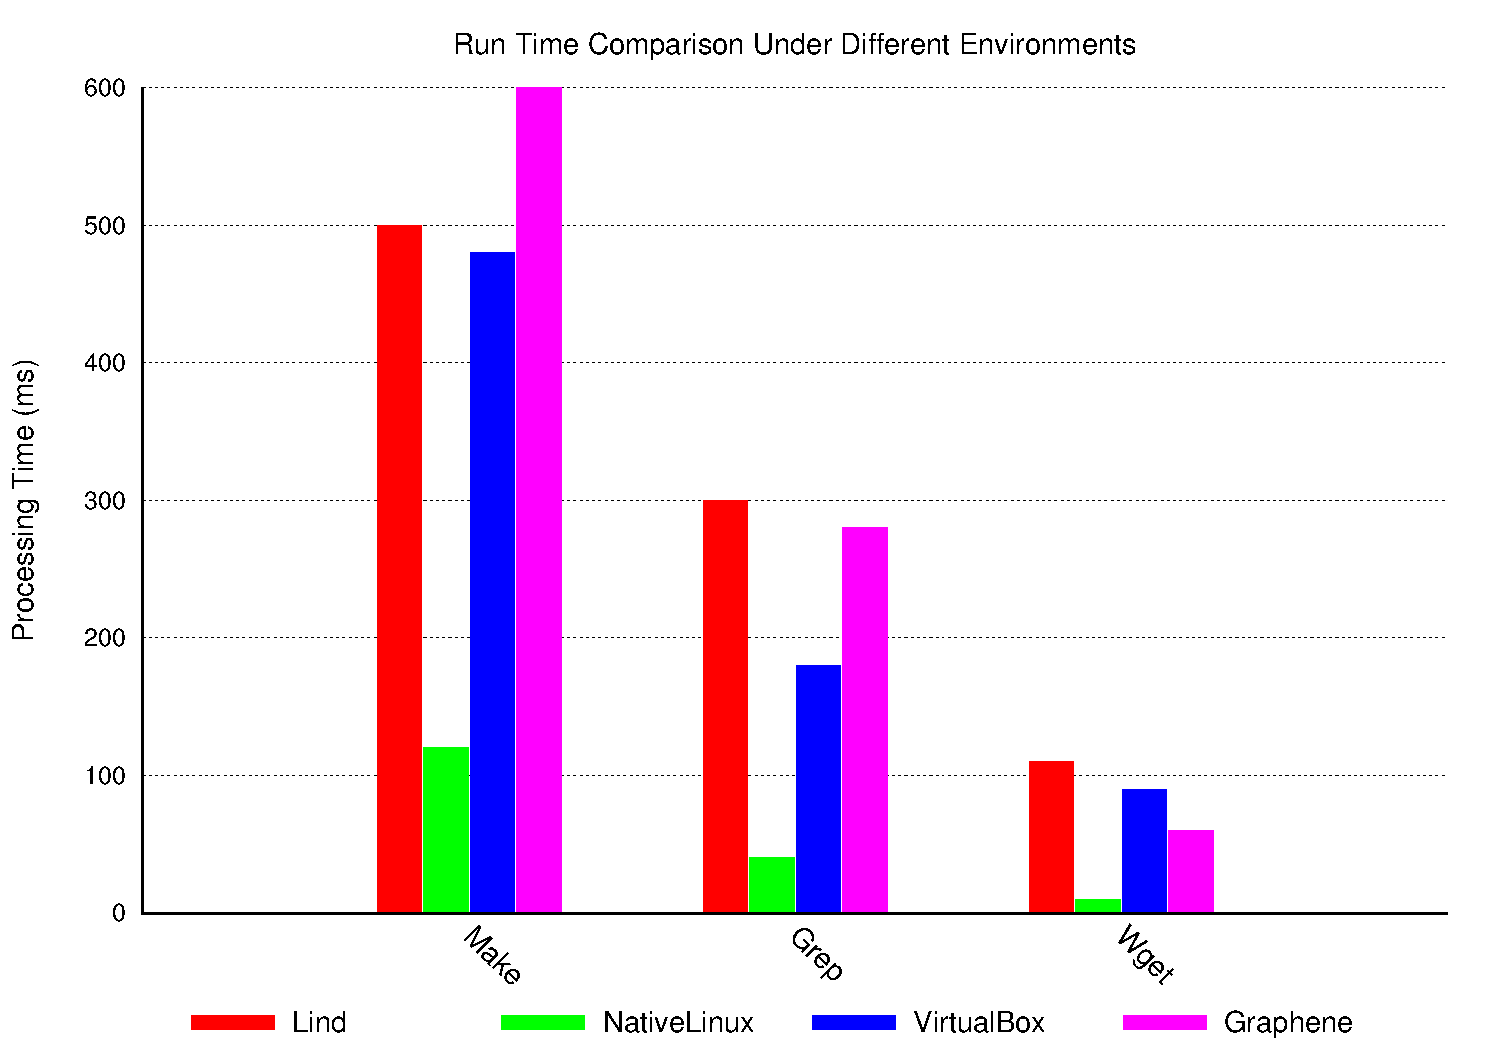
\includegraphics[width=1.0\columnwidth]{diagram/lind_ccs15_diagram_05.pdf}
\caption{Performance Evaluation Results}
\label{fig:performance_evaluation_results}
\end{figure}

\subsection{Conclusion}
Through our security evaluation and performance evaluation, we can see that 
Lind indeed achieved stronger security, compared against other systems.

Our metric is effective in creating new designs concerning interaction and contacting with the kernel. 
More general, we can conclude that new designs using our metric are likely to be better. 